\documentclass[a4paper,12pt]{article}
\renewcommand{\baselinestretch}{1.5}
\usepackage[utf8]{inputenc}
\usepackage{multirow}
\usepackage{booktabs}
\usepackage{tabularx}
\usepackage{fullpage}
\usepackage{geometry}
\usepackage[labelfont=bf]{caption}
\usepackage{graphicx}
\usepackage{siunitx}
\usepackage{float}
\usepackage{natbib}
\usepackage{url}
\usepackage[english]{babel}
\usepackage{blindtext}
\usepackage{csquotes}
\usepackage[numbered,framed]{matlab-prettifier}
\usepackage{color}
\usepackage{amsmath}
\usepackage{amssymb}
\usepackage{bbm}
\usepackage{framed}
\usepackage{hyperref}
\usepackage{subcaption}
\usepackage{titlesec}

\setcounter{secnumdepth}{4}
\renewcommand{\topfraction}{0.85}
\renewcommand{\bottomfraction}{0.85}
\renewcommand{\textfraction}{0.15}
\renewcommand{\floatpagefraction}{0.7}

\title{\textbf{Digital Tools For Finance}\\ Final Assignment}

\author{\\ZIFENG TANG(21-742-093)\\ YUZHI MAO(21-742-218)\\HAORAN ZHU(21-742-069)\\ }
\date{Due date: 19th December 2022}
\geometry{left=27mm,right=27mm,top=35mm,bottom=30mm,headheight=15pt}
\begin{document}


\maketitle
\newpage
\tableofcontents
\newpage
\section{Introduction}
\subsection{Risk Measures}
\subsubsection{Standard Deviation, Semi Variance, Lower Partial Moment Index}
Standard deviation is the most commonly used risk measurement indicator in not only industry but also academic research study. In the 1950s, Markowitz used the expected rate of return, variance and covariance to determine the efficient frontier of investment. Each portfolio on the boundary either maximizes its expected return given the variance, or has a minimized variance given a target rate of return. In later studies, many scholars found that investors' views on risk are not symmetrical, instead, they pay more attention to the downside risk of financial assets. Later, \cite{MH1991} further proposed two indicators to measure the downside risk: mean downside semi variance $\text{SV}_{m}$ and target downside semi variance $\text{SV}_{t}$:
\begin{equation}
\begin{aligned}
    \text{SV}_{m} &= \frac{1}{T} \sum_{t=1}^T \max \left[0, E(R_{t})-R_{t}\right]^2 \\
    \text{SV}_{m} &=\frac{1}{T} \sum_{t=1}^T \max \left[0, R^*-R_t\right]^2
\end{aligned}        
\end{equation}

\noindent 
where $E(R_{t})$ is the average rate of return, and $R^*$ is the target rate of return.
The above indicators assigned a great impact on asset portfolio theory, but they have also caused great controversy on the description of the skewness of the financial asset distribution.
\cite{BV1975} first proposed the concept of lower partial moment, LPM, which defined as follow:
\begin{equation}
 \begin{aligned}
    \text{LPM}(a, t)=\frac{1}{T} \sum_{t=1}^T \max \left[0,\left(R^*-R_t\right)\right]^a
\end{aligned}       
\end{equation}
\noindent 
where $a$ is the order of the lower partial moment, and $R^*$is the target rate of return. 1) When $a=0$, LPM represents the probability lower than the target rate of return; 2) When $a=1$, LPM is the average value that is lower than the target rate of return. This indicator can then be used to represent risk-neutral investors; 3) When $a=2$, LPM is the risk below the target rate of return, which can be used to describe risk-averse investors; 4) As $a$ increases, investors become more risk averse. Following a long period of time, the method of determining the order $a$ of LPM has attracted great attention from the academic community, and many related algorithms and research on the properties of LPM have been fast developed.

\subsubsection{Value at Risk Indicators}
Besides the risk metrics mentioned above, J. P. Morgan introduced the concept of VaR in 1994 in response to the financial disasters of the 1990s. It is defined as follows
\begin{equation}
\operatorname{VaR}_\alpha(X)=-q_\alpha(X)=-\inf \{x: P[X \leq x] \geq \alpha\}    
\end{equation}
where $X$ is a given random variable, and $\alpha$ is the confidence level.
This indicator was widely noticed by researchers and practitioners at that time. However, with the in-depth of research, this indicator has been questioned a lot. It does not meet the consistency condition of risk measurement indicators proposed by \cite{AP1999Coherentmeasures}, so it cannot measure the tail risk and the risk of occurrence of the extreme events. \cite{AP1999Coherentmeasures} proposed a new risk measurement indicator called conditional value at risk CVaR, which is defined as the following
\begin{equation}
 \operatorname{CVaR}_\alpha(X)=-E\left[X \leq q_\alpha(X)\right]   
\end{equation}
where $X$ is required to be a continuous random variable. This indicator can make up for the disadvantage of VaR, because it is consistent and compatible, and can better measure the tail risk. \cite{RR2002}believed that another defect of VaR index is that it cannot describe the degree of loss after the loss exceeds the critical value of the index. It only provides a minimum limit for the loss at the tail of the loss distribution with optimism rather than following the conservatism that prevails in risk management. Additionally, they believe that compared with VaR, the advantages of CVaR indicators include its subadditivity, measurability of risks exceeded VaR, and ability to solve the optimization problem of large-scale asset portfolios. However, CVaR is no longer a consistent measure of risk whenever the density of loss function is not continuous. Therefore, \cite{TD2002} brought up the concept of Expected Shortfall $ES$:
\begin{equation}
 ES(\alpha)=\frac{\int_0^\alpha \operatorname{VaR}(u) du}{\alpha}    
\end{equation}
This indicator overcomes the disadvantages of $\text{CVaR}_{\alpha}(X)$, and has been widely used in practice.
\subsection{Risk Parity Model}
Markowitz model represents a new stage of the development of modern portfolio theory. The model has been improved by scholars with respect to strong parameter sensitivity and insufficient risk measurement. At the same time, many scholars and practitioners began to focus on other asset portfolio models.\\
Bridgewater Associates first proposed the idea of risk parity in 1996, and created the All Weather(AW) strategy. The core idea of the model is to equates the risk of each asset by determining their weights in the asset portfolio. The total risk $\boldsymbol{\mathcal{R}}_\mathbf{p}(\vec{w})$ of a portfolio can be written as:
 \begin{equation}
\boldsymbol{\mathcal{R}}_{\mathbf{p}}=\sqrt{\vec{w}^T \Sigma \vec{w}}  
 \end{equation}
The marginal risk $\boldsymbol{M}\boldsymbol{\mathcal{R}}(X_{i})$ and the risk contribution $\boldsymbol{\mathcal{R}}\boldsymbol{C}(X_{i})$ of each asset $i$ to the portfolio can be written as:
\begin{equation}
\begin{aligned}
\boldsymbol{M}\boldsymbol{\mathcal{R}}\left(X_i\right)&=\frac{\partial \boldsymbol{\mathcal{R}}_{\mathbf{p}}}{\partial w_i}\\
\boldsymbol{\mathcal{R}}\boldsymbol{C}\left(X_i\right)&=w_i \frac{\partial \boldsymbol{R}_\mathbf{p}}{\partial w_i}=w_i \frac{(\Sigma \vec{w})_i}{\sqrt{\vec{w}^T \sum \vec{w}}}  
    \end{aligned}
\end{equation}
Later, \cite{QE2002} conducted an empirical analysis using the Russell 1000 Index and the Exchange Traded Funds, and found that the performance of the investment portfolio based on the risk parity model was significantly better than that of a single financial asset. At the same time, the strategy obtained by the risk parity model has a higher average rate of return and Sharpe ratio, which proves that the risk parity model can disperse risks and improve the robustness of returns.
\section{Calculate Risk Measures based on Multivariate t-distribution (MVT)}
\subsection{Data Description and Normality Test}
\subsubsection{Data Selection}
In order to conduct empirical analysis, we use the daily trading data of CSI 300, CSI Aggregate Bond Index and Gold Exchange Traded Fund to represent the performance of stock, marketable Securities, and commodity markets, respectively. Through the data of the daily closing price from 2015 to 2019, we can calculate the respective daily average return according to $r_{t}=\frac{P_{t}-P_{t-1}}{P_{t}}$ and draw the following figure.
\begin{figure}[H]
    \centering
    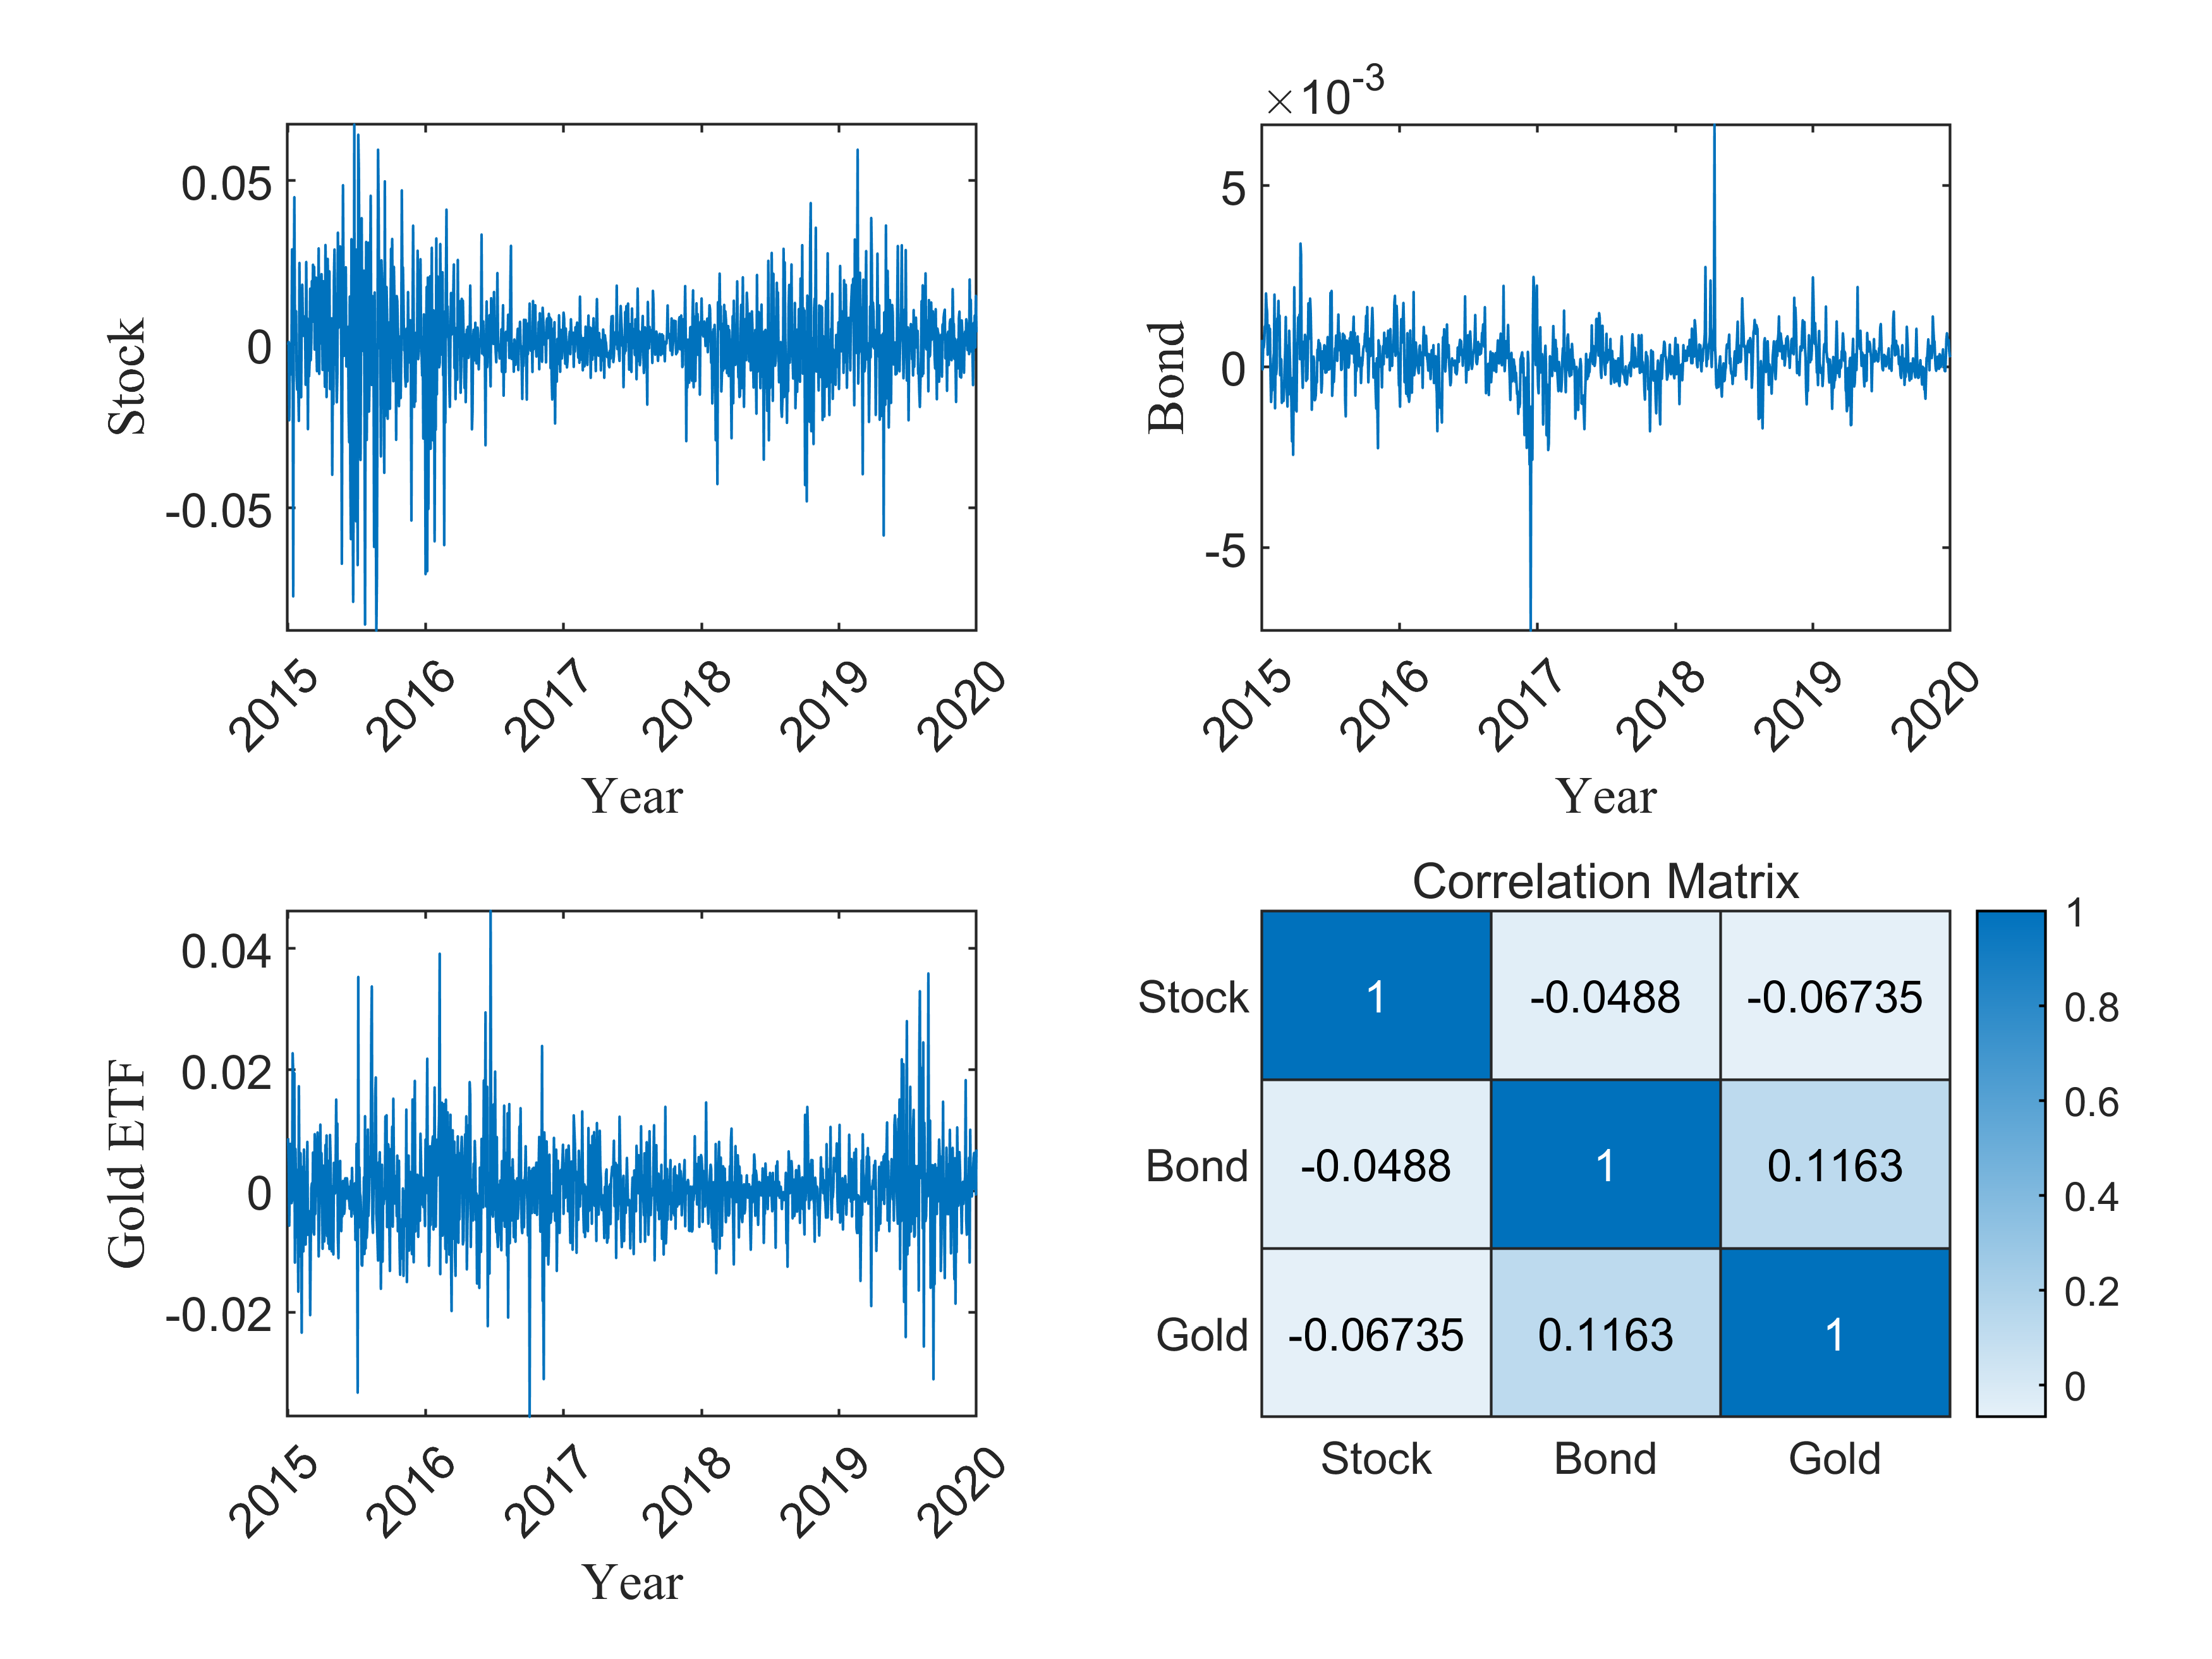
\includegraphics[scale=1]{Figure/FIG1-Daily-Return.png}
    \caption{The Daily Return of CSI-300 (upper left), CSI-ABI (upper right), and
Gold-ETF (lower left) and Correlation Matrix (lower right) from 2015 to 2019}
    \label{Fig1}
\end{figure}

\subsubsection{Statistics Description and Normality Test}
Through calculation, various statistics of the daily return rate of CSI 300, CSI Aggregate Bond Index(ABI) and Gold Exchange Traded Fund(ETF) can be obtained, which are listed as follows:
\begin{table}[H]
\centering
\begin{tabular}{|c|c|c|c|c|c|c|c|}
\hline
{\bf Mean} &  {\bf Std} & {\bf Median} &  {\bf Max} &  {\bf Min} & {\bf Kurtosis} & {\bf Skewness} & {\bf J-B Test} \\
\hline
    0.02\% &     1.54\% &     0.05\% &     6.71\% &    -8.75\% &      8.96  &     -0.85  &      0.001 \\
\hline
    0.02\% &     0.07\% &     0.02\% &     0.67\% &    -0.73\% &     16.87  &     -0.40  &      0.001 \\
\hline
    0.03\% &     0.75\% &     0.04\% &     4.63\% &    -3.73\% &      7.75  &      0.46  &      0.001 \\
\hline
\end{tabular}  
\caption{The Statistics Description of CSI 300, CSI ABI, and Gold ETF }
\label{Tab1}
\end{table}

\begin{figure}[H]
    \centering
    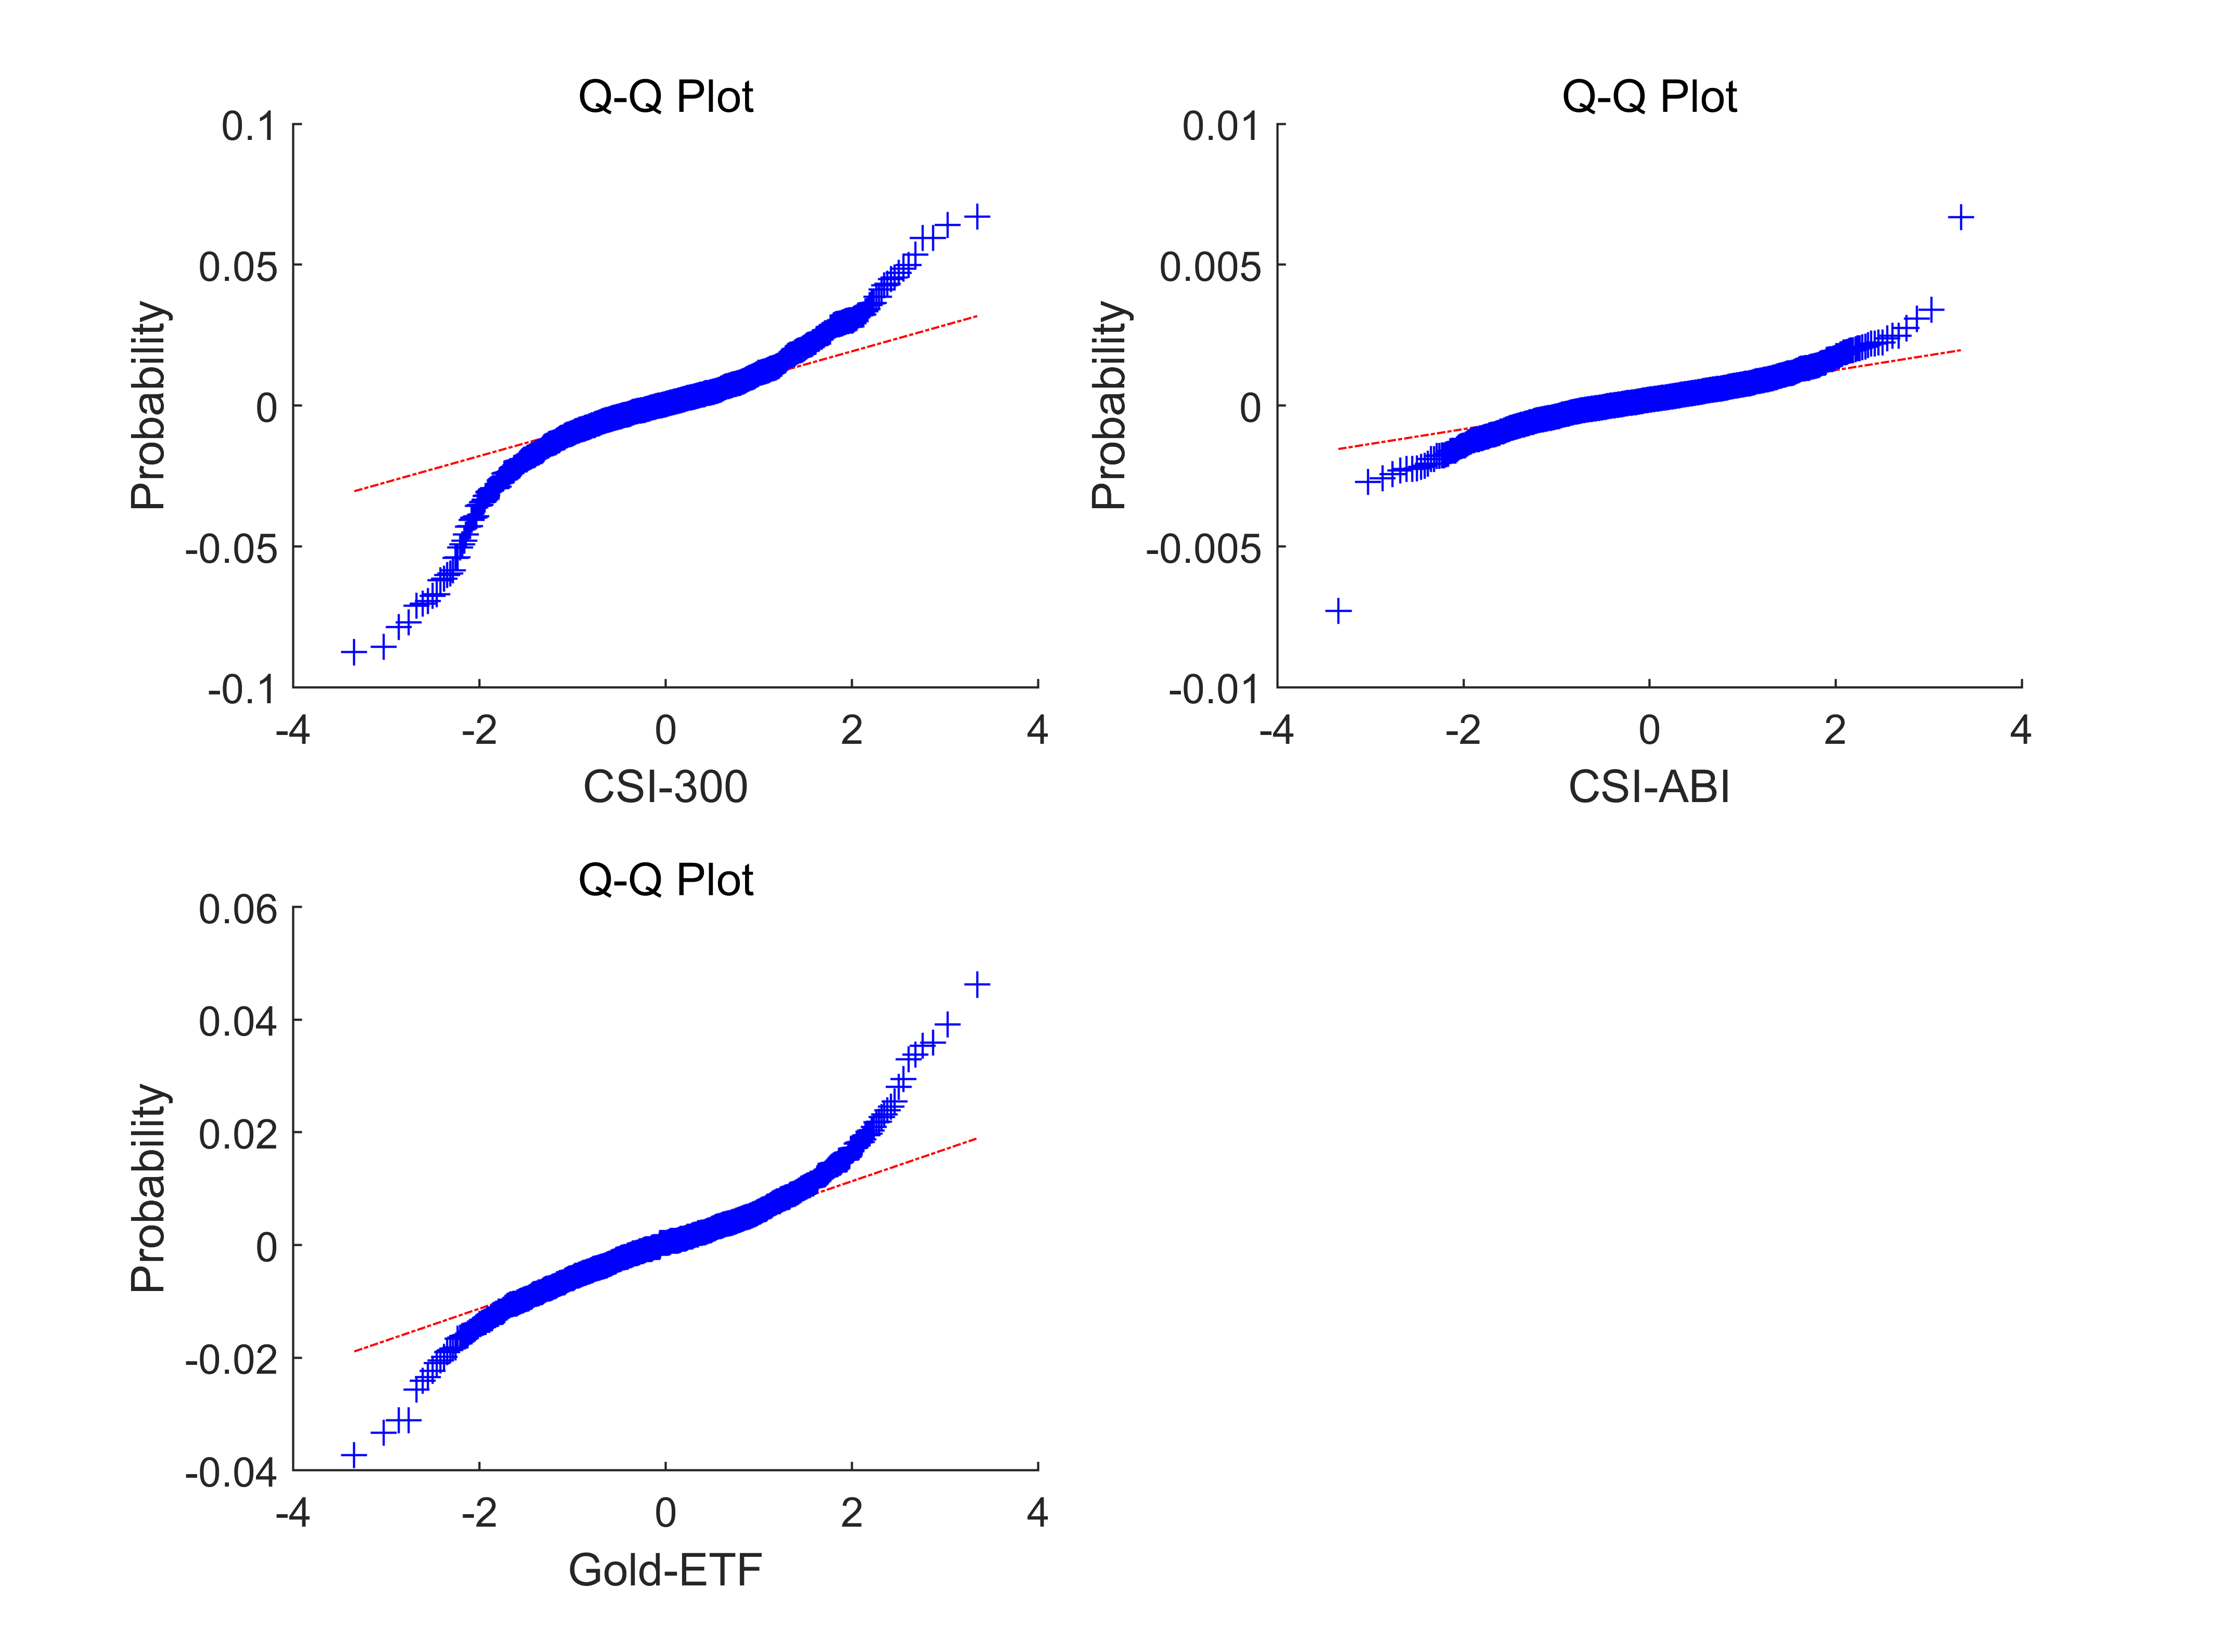
\includegraphics[scale=0.8]{Figure/FIG2-Q-Q.png}
    \caption{The Q-Q Plot of CSI-300 (upper left), CSI-ABI (upper right), and
Gold-ETF (lower left) daily return of year 2015-2019}
    \label{Fig2}
\end{figure}

\noindent According to the above results, we can draw the following conclusions:
\begin{itemize}
    \item[1)] \textbf{Volatility}: The standard deviation(SD) of the CSI 300 Index is higher than that of the Gold ETF and much higher than that of the CSI ABI. It indicates that the volatility of the stock market is high, while that of the bond market is low, and the volatility of the gold market is in the middle.
    \item[2)] \textbf{Leptokurtic}: We found that the three types of assets all have high kurtosis, i.e., greater than 3, which shows that their logarithmic returns have a "fat tail" phenomenon. At the same time, the CSI 300 Index and the CSI ABI have a certain "negative bias", while the Gold ETF has a certain "positive bias". Therefore, we found that the logarithmic return series of the three types of assets all have "peak and fat tail".
    \item[3)] \textbf{Normality Test}: According to the fact that the p-value of the Jarque–Bera test(JB test) of the three assets is less than 0.05, it can be seen that at the $95\%$ confidence level, the original hypothesis of "H0: the logarithmic return follows a normal distribution" is rejected, which shows that the logarithmic return of the three assets does not follow the normal distribution. In addition, the corresponding Q-Q Plot can intuitively show this characteristic.
\end{itemize}

\subsection{Parameter Estimation of MVT Distribution}
The density function of the $d$-dimensional Student $t$ distribution $T_\nu(\mu, \Sigma)$ with $v>$ 0 degrees of freedom, location paramter $\mu \in \mathbb{R}^d$ and symmetric, positive definite scatter matrix $\Sigma \in \operatorname{SPD}(\mathrm{d})$ is given by
\begin{equation} \label{E1.1}
p(x \mid v, \mu, \Sigma)=\frac{\Gamma\left(\frac{d+v}{2}\right)}{\Gamma\left(\frac{v}{2}\right) v^{\frac{d}{2}} \pi^{\frac{d}{2}}|\Sigma|^{\frac{1}{2}}} \frac{1}{\left(1+\frac{1}{v}(x-\mu)^{\mathrm{T}} \Sigma^{-1}(x-\mu)\right)^{\frac{d+v}{2}}}
\end{equation}
which is often used to describe the distribution of returns on multiple financial assets, because it can reflect the characteristics of "peaks and fat tails" and the correlation of returns on different assets.
\\ \noindent According to the relevant statistical analysis of the daily return of the three types of assets in \textbf{Figure \ref{Fig2}}, we know that using the normal distribution to describe the return on financial assets is not effective and there are correlations between the return on each asset, so it is rational to use the MVT distribution to estimate the rate of return of the three major assets. Through the MMF method introduced by \cite{hasannasab2021alternatives}, we can obtain the estimated parameters as follow
$$
\hat{\nu}=3.4273,\:\hat{\mu}=[8.519,1.783,2.064]\times 10^{-4}
$$
$$
\hat{\Sigma}=\begin{bmatrix}
  998 &  -2.55 &  -7.24 \\
 -2.55 &   2.59 &   3.25 \\
 -7.24 &   3.25 &   279 \\    
\end{bmatrix} \times 10^{-7}
$$
\begin{figure}[H]
    \centering
    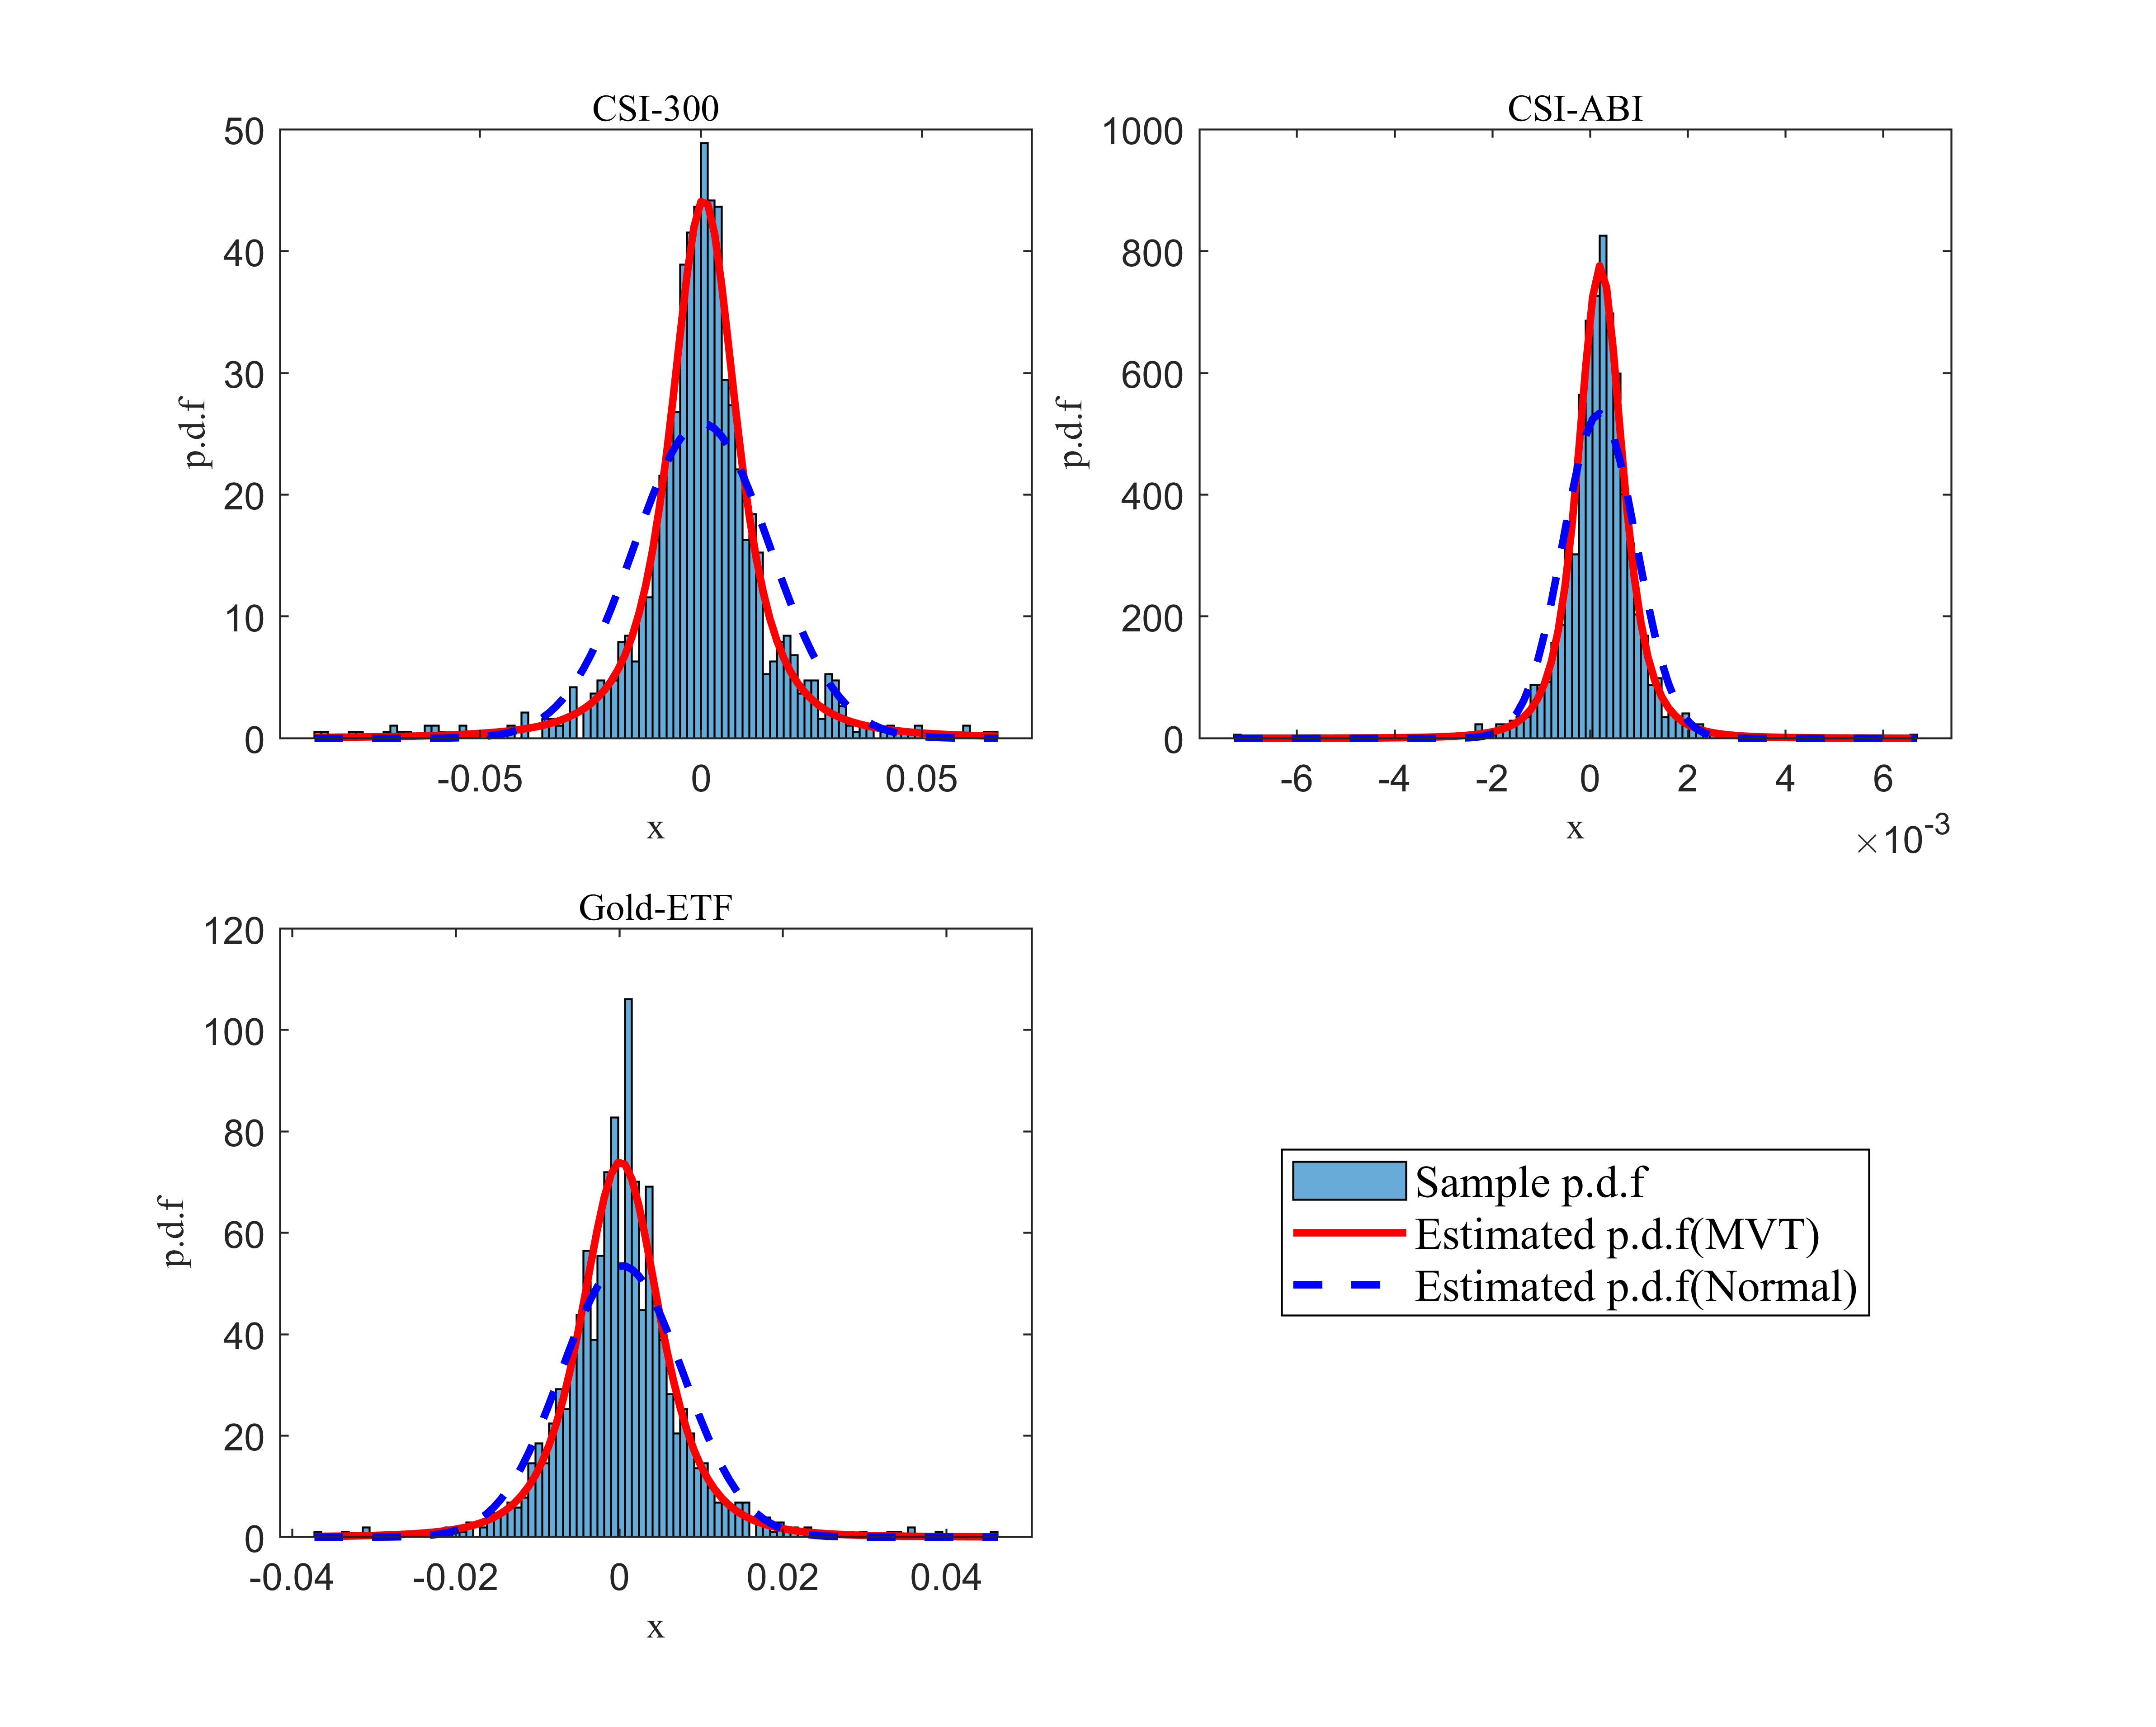
\includegraphics[scale=0.8]{Figure/FIG3-PDF.png}
    \caption{The p.d.f of CSI-300 (upper left), CSI-ABI (upper right), and
Gold-ETF (lower left)}
    \label{Fig3}
\end{figure}
\subsection{VaR and ES based on MVT}
\subsubsection{Theoretical Formula}
Assume the return $r=(r_1,r_2,r_3)^T \sim t_{\nu}(\mu,\Sigma)$ is a 3-variate t-distribution random variable, then the return of a portfolio with weight $w=(w_1,w_2,w_3)^T$ is $r_p(w)=w^Tr \sim t_{\nu}(w^T\mu,w^T\Sigma w)$. Denote $\mu_p(w)=w^T\mu$ and $\sigma_p^2(w)=w^T\Sigma w$, then the $\text{VaR}_{\alpha}$ and $\text{ES}_{\alpha}$ of the portfolio are
\begin{equation} \label{E2.3}
\begin{aligned}
\text{VaR}_{\alpha}\left(r_p(w)\right) &= \mu_p(w) +\Sigma_p(w) t_{\nu}^{-1}(\alpha)    \\
\text{ES}_{\alpha}\left(r_p(w)\right) &= \mu_p(w) +\Sigma_p(w) \text{ES}_{\alpha}\left(t\right) \\
&=\mu_p(w) -\Sigma_p(w) \frac{f_{t_{\nu}}\left(t^{-1}_\alpha(\nu)\right)}{F_{t_{\nu}}\left(t^{-1}_\alpha(\nu)\right)} \cdot \frac{\left(\nu+(t^{-1}_\alpha(\nu))^2\right)}{\nu-1}
\end{aligned}
\end{equation}
where $t \sim t_{\nu}(0,1)$ and $f_{\nu}(x),\:F_{\nu}(x)$ are the p.d.f and c.d.f of t respectively.

\subsubsection{Monte Carlo Simulation}
Combined with the method in \textbf{3.2}, we can compare the estimation effect of risk measurement indicators based on MVT and normal distribution through the Monte Carlo Simulation. We construct a portfolio with weight $w=[1/3,1/3,1/3]$ and calculated the Expected Shortfall and Value at Risk based on real data, estimated normal distribution and estimated MVT respectively. The error rate of estimation and box plot of the errors are given as follow
\begin{table}[H]
    \centering
    \begin{tabular}{|c|c|c|}
    \hline
    {\bf Risk Measure} &  {\bf VaR} &   {\bf ES} \\
    \hline
    {\bf Real Value} &    -0.81\% &    -1.37\% \\
    \hline
    {\bf Estimated Value (MVT)} &    -0.80\% &    -1.27\% \\
    \hline
    {\bf Error Rate} &     1.23\% &     7.30\% \\
    \hline
    {\bf Estimated Value (Normal)} &    -0.89\% &    -1.12\% \\
    \hline
    {\bf Error Rate} &    -9.88\% &    18.25\% \\
    \hline
    \end{tabular}  
    \caption{The Estimated VaR and ES based on MVT and Normal Distribution}
    \label{Tab2}
\end{table}
\begin{figure}[H]
    \centering
    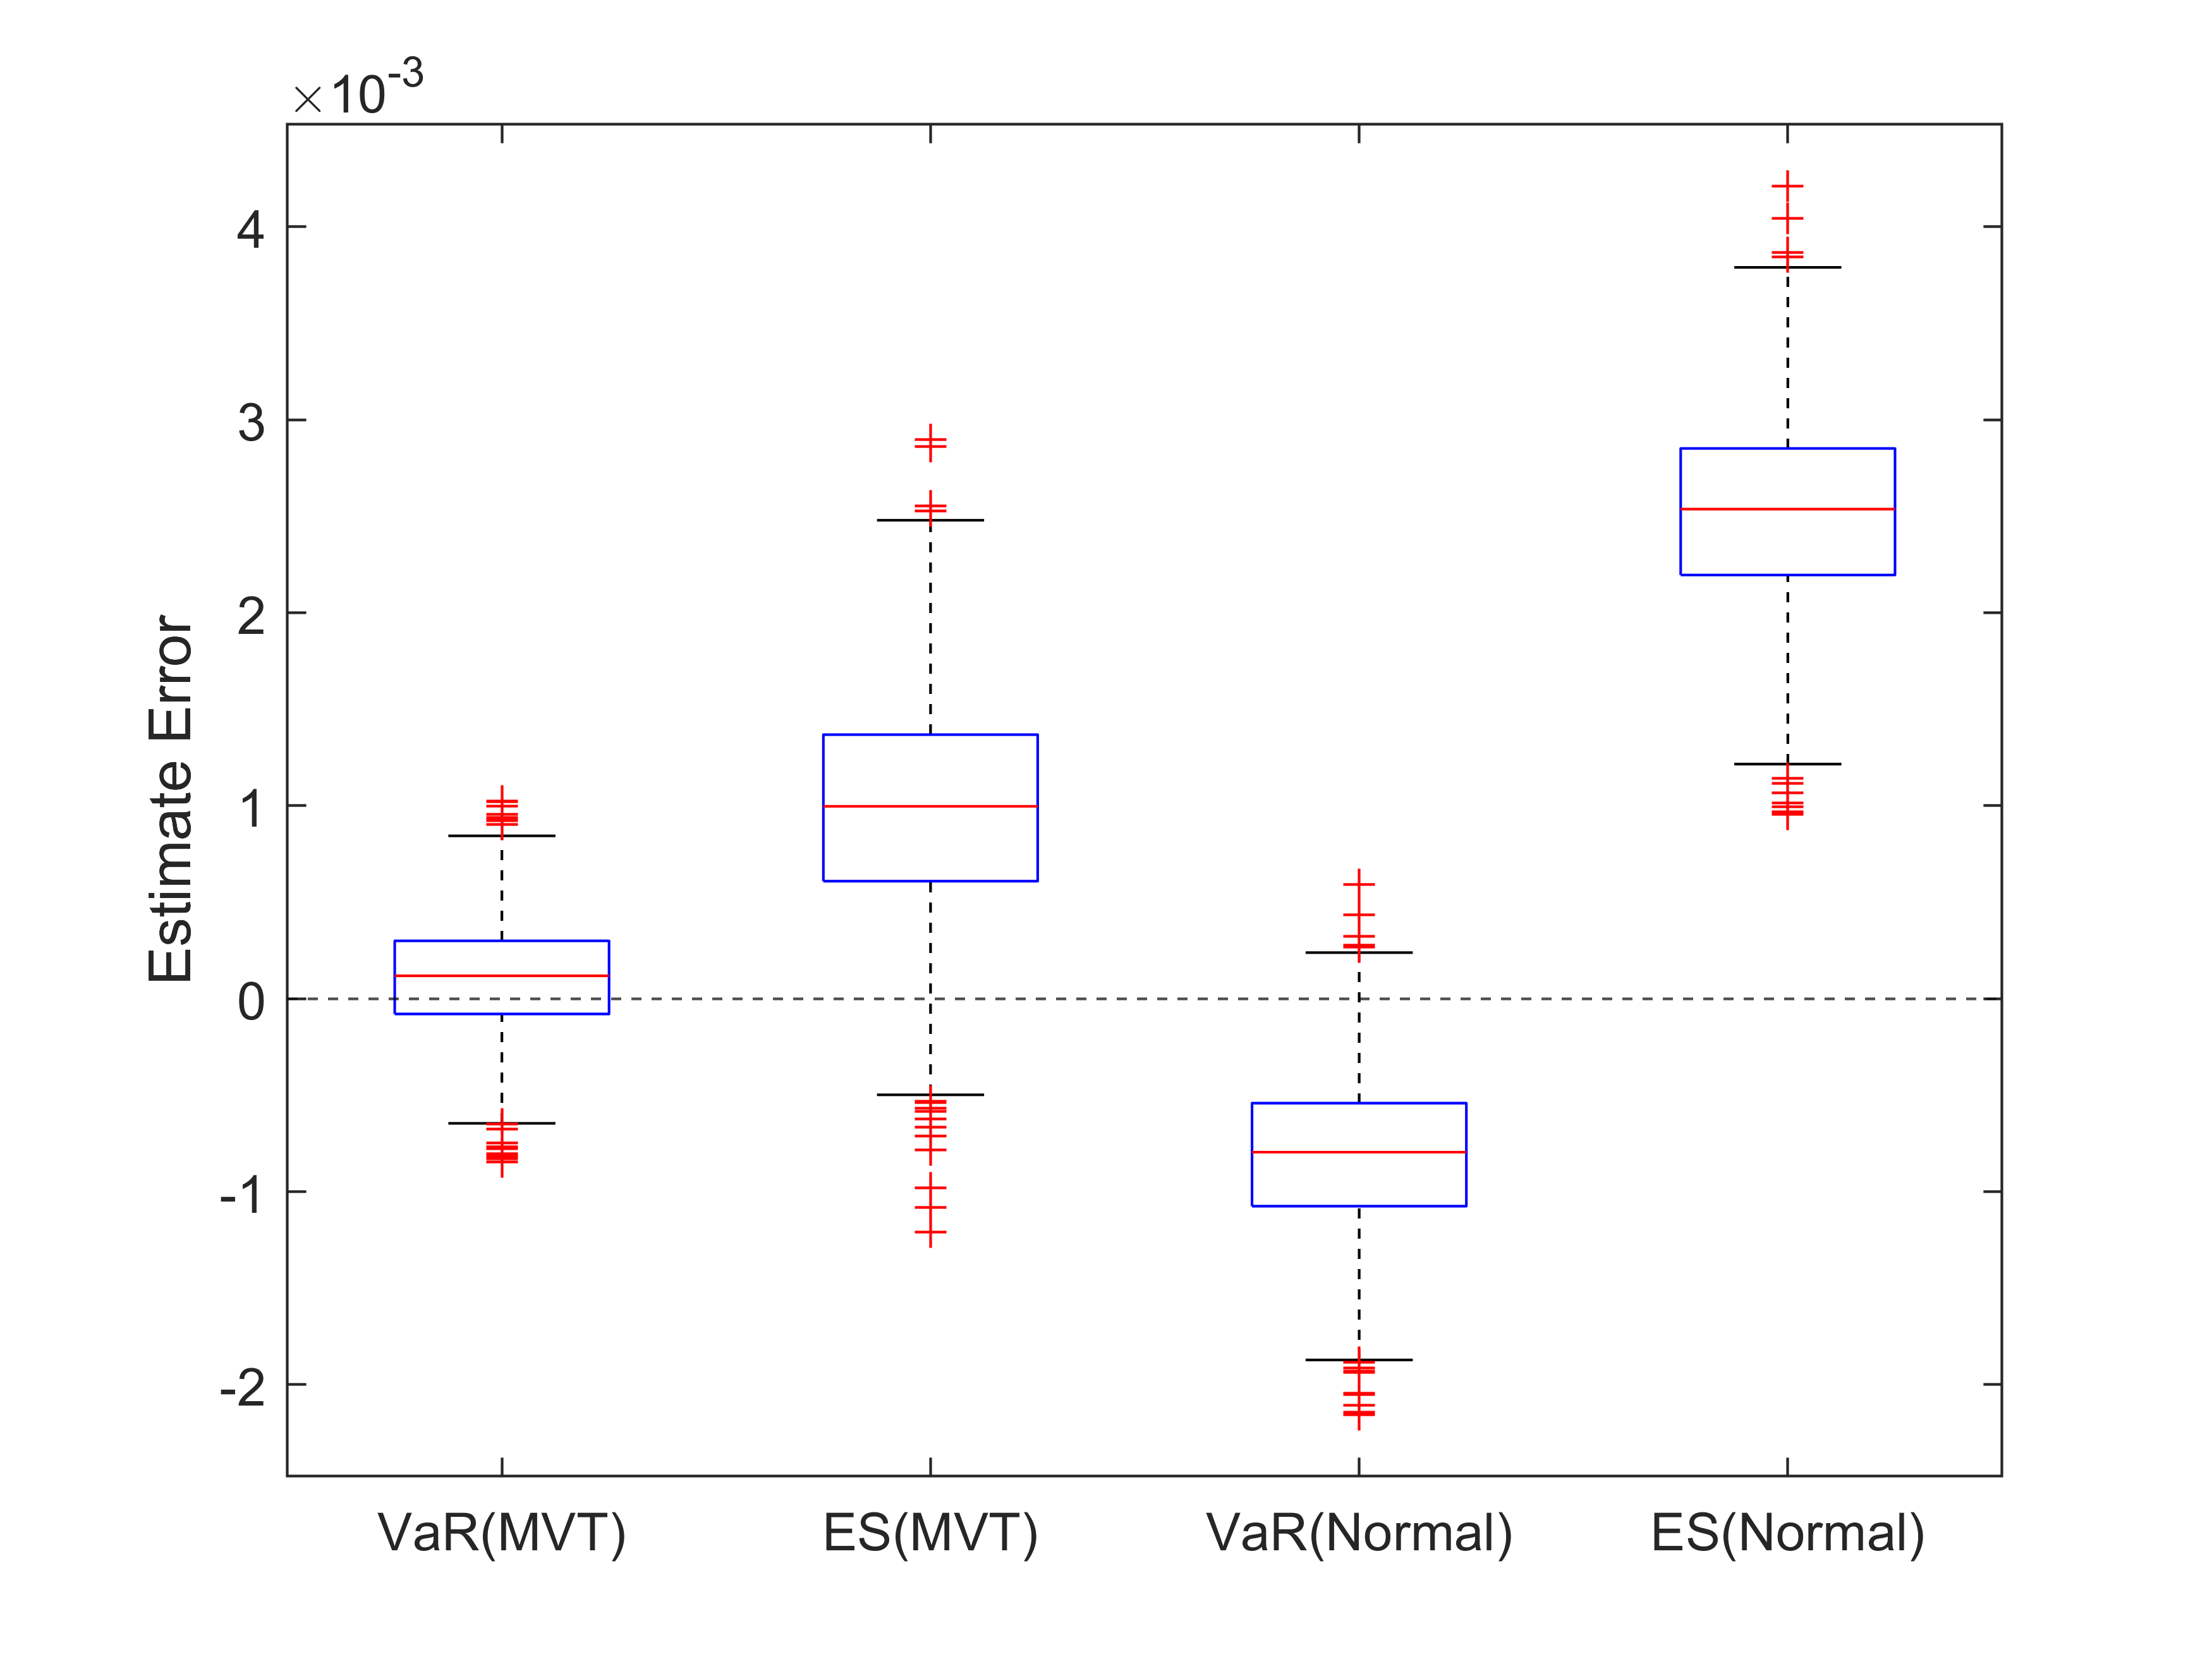
\includegraphics[scale=0.9]{Figure/FIG4-MC.png}
    \caption{The Estimate Error of VaR and ES based on MVT and Normal Distribution}
    \label{Fig4}
\end{figure}
From \textbf{Figure \ref{Fig4}}, we can conclude that the errors of VaR and ES estimated based on MVT are smaller than those based on Normal.
\section{Risk Parity Model Based on MVT}
\subsection{Data Selection}
In order to test whether the risk parity model based on MVT can perform well in the actual market, we use the standard deviation(Std), value at risk(VaR), and expected shortfall(ES) as the indicators of risk measurement to construct the risk parity model for CSI 300, CSI ABI and Gold ETF and carry out the dynamic backtesting. In terms of the time duration, we still applied the logarithmic rate of return data from 2015 to 2019. However, due to the need to estimate parameters and calculate risk metrics during the backtesting process, the actual backtesting interval is from March 2015 to December 2019.

\subsection{Model Derivation}
\subsubsection{Consistency in Risk Metrics}
\cite{AP1999Coherentmeasures} gave the concept of consistency of risk measurement: Let $\Omega$ be the set of all possible states of an event, the set $\mathcal{F}$ of all real-valued functions defined on $\Omega$ is called the risk set. The risk measure $\boldsymbol{\mathcal{R}}(.)$ is a mapping from $\mathcal{F}$ to space $\mathbb{R}$. The risk measure is consistent if it satisfies the following properties: 
\begin{itemize}
  \item Monotonicity: $\forall X_1 \geq X_2 \in \mathcal{F}, \mathcal{R}\left(\mathrm{X}_1\right) \geq \mathcal{R}\left(\mathrm{X}_2\right)$ 
  \item Homogeneity: $\forall X \in \mathcal{F}, c \geq 0, \mathcal{R}(\mathrm{cX})=c \mathcal{R}(\mathrm{X})$
  \item Translation Invariance: $\forall X \in \mathcal{F}, c \in \mathbb{R}, \mathcal{R}(\mathrm{X}+\mathrm{c})=\mathcal{R}(\mathrm{X})-c$ 
  \item Subadditivity: $\forall X_1, X_2, \ldots, X_N \in \mathcal{F}, \mathcal{R}\left( \sum_{i=1}^{N} X_i\right) \leq \sum_{i=1}^{N} \mathcal{R}\left(X_i\right)$
\end{itemize}
% \noindent(1) Monotonicity: $\forall X_1 \geq X_2 \in \mathcal{F}, \mathcal{R}\left(\mathrm{X}_1\right) \geq \mathcal{R}\left(\mathrm{X}_2\right)$ \\
% (2) Homogeneity: $\forall X \in \mathcal{F}, c \geq 0, \mathcal{R}(\mathrm{cX})=c \mathcal{R}(\mathrm{X})$ \\
% (3) Translation Invariance: $\forall X \in \mathcal{F}, c \in \mathbb{R}, \mathcal{R}(\mathrm{X}+\mathrm{c})=\mathcal{R}(\mathrm{X})-c$ \\
% (4) Subadditivity: $\forall X_1, X_2, \ldots, X_N \in \mathcal{F}, \mathcal{R}\left( \sum_{i=1}^{N} X_i\right) \leq \sum_{i=1}^{N} \mathcal{R}\left(X_i\right)$

\noindent Whether the risk measurement indicators are consistent plays a vital role in measuring the risk degree of the asset portfolio. Use N assets $X_{1}, X_{2},...X_{N}$ to build an asset portfolio $w=(w_{1},w_{2},...,w_{N} )^T$, where $\sum_{i=1}^N w_i=1$. If the risk measurement index $\mathcal{R}(.)$ has subadditivity and homogeneity, then
$$
    \mathcal{R}\left(\sum_{i=1}^N w_i X_i\right) \leq \sum_{i=1}^N w_i \mathcal{R}\left(X_i\right)
$$
which investors can reduce investment risk by allocating funds in different assets. By definition, the standard deviation is consistent, and the consistency of the expected loss has been proved by \cite{TD2002}.


\subsubsection{Model Extension}
The traditional risk parity model is based on the standard deviation, We now consider extended models based on different risk measures. From \textbf{Equation (\ref{E2.3})}, the risk contribution can be calculated as below:
\begin{itemize}
    \item[(M1)] \textbf{Model based on Standard Deviation}
    \begin{equation}
     \boldsymbol{\mathcal{R}}\boldsymbol{C}\left(X_i\right)=w_i \frac{\partial \boldsymbol{\mathcal{R}}_{\boldsymbol{p}}}{\partial w_i}=w_i \frac{(\Sigma \vec{w})_i}{\sqrt{\vec{w}^T \sum \vec{w}}}   
    \end{equation}

    \item[(M2)]\textbf{Model based on $\text{VaR}_{\alpha}$}
    \begin{equation}
     \boldsymbol{\mathcal{R}}\boldsymbol{C}\left(X_i\right)=-w_i\mu_{i} - w_i \frac{(\Sigma \vec{w})_i}{\sqrt{\vec{w}^T \sum \vec{w}}}t_{\nu}^{-1}(\alpha)  
    \end{equation}
    \item[(M3)]\textbf{Model based on $\text{ES}_{\alpha}$}
    \begin{equation}
     \boldsymbol{\mathcal{R}}\boldsymbol{C}\left(X_i\right)=-w_i\mu_{i} + w_i \frac{(\Sigma \vec{w})_i}{\sqrt{\vec{w}^T \sum \vec{w}}}\frac{f_{t_{\nu}}\left(t^{-1}_\alpha(\nu)\right)}{F_{t_{\nu}}\left(t^{-1}_\alpha(\nu)\right)} \cdot \frac{\left(\nu+(t^{-1}_\alpha(\nu))^2\right)}{\nu-1} 
    \end{equation}
\end{itemize}
where we choose the absolute value of VaR and ES in \textbf{Equation \ref{E2.3}} to calculate risk contribution. Then the generalized model would be equivalent to the following optimization problem
\begin{equation}
\begin{aligned}
 w_p=&\underset{w \in \mathbb{R}^d}{\text{argmin}} \sum_{i \neq j} \left(\boldsymbol{\mathcal{R}}\boldsymbol{C}\left(X_i\right)-\boldsymbol{\mathcal{R}}\boldsymbol{C}\left(X_j\right)\right)^2\\
 & \text{s.t.} \: \|w\|=1,\: w_i\ge 0,\:i=1,2,\dots,d
\end{aligned}
\end{equation}



\subsection{Model Backtesting}
We use the method of quarterly rebalancing for backtesting. There are 1, 2, ..., 19 quarters in total. When repositioning for time $t$, the following steps are performed:
\begin{enumerate}
    \item \textbf{Calculate the parameters of MVT and the risk measures each asset in the $\boldsymbol t^{\boldsymbol t\boldsymbol h}$ quarter.} Based on the historical data prior to the $t^{th}$ quarter (half year), we first use the MMF method to estimate the distribution parameters of the $t^{th}$ quarter. Then, we use the distribution parameters of MVT to calculate the the risk measures, i.e., value at risk(VaR) and expected shortfall(ES), of various assets in the $t^{th}$ quarter.
    \item \textbf{Use the risk parity model to calculate the weight of each asset $\boldsymbol w_{\boldsymbol t} \boldsymbol = \boldsymbol (\boldsymbol w_{\boldsymbol 1}, \boldsymbol w_{\boldsymbol 2}, \boldsymbol w_{\boldsymbol 3}\boldsymbol )^{\boldsymbol T}$ in period t} that equates the risk contribution of all assets.
    \item \textbf{Rolling backtest.} Calculate the indicators used to evaluate the performance of the models.
\end{enumerate}

\subsection{Result analysis}
\subsubsection{Evaluation Index}
\begin{table}[H]
    \centering
   \begin{tabular}{|c|c|c|c|c|}
    \hline
    {\bf Index} & {\bf Annual Return} &  {\bf Std} &  {\bf MDD} & {\bf Sharp Ratio}  \\
    \hline
    {\bf std Model} &     5.39\% &     1.83\% &     4.00\% &    1.3080    \\
    \hline
    {\bf VaR Model} &     5.25\% &     1.71\% &     3.94\% &    1.3157   \\
    \hline
    {\bf ES Model} &     5.28\% &     1.73\% &     3.94\% &    1.3161   \\
    \hline
    {\bf CSI 300} &     0.23\% &    23.86\% &    61.71\% &   -0.1159    \\
    \hline
    {\bf CSI ABI} &     4.81\% &     1.15\% &     4.47\% &    1.5745   \\
    \hline
    {\bf GOLD ETF} &     7.79\% &    11.50\% &    15.64\% &    0.4167  \\
    \hline
    \end{tabular}  
    \caption{The Evaluation Indexes of Models and Assets (Apr,2015-Dec,2019),$R_f=3\%$}
    \label{Tab3}
\end{table}

\subsubsection{Asset Allocation Weight}
\begin{table}[H]
    \centering
    \begin{tabular}{|c|c|c|c|}
    \hline
    {\bf Model} & {\bf SCI 300} & {\bf SCI ABI} & {\bf Gold ETF} \\
    \hline
    {\bf Std Model} &     5.91\% &    84.32\% &     9.77\% \\
    \hline
    {\bf VaR Model} &     5.27\% &    86.92\% &     7.81\% \\
    \hline
    {\bf ES Model} &     5.35\% &    86.50\% &     8.15\% \\
    \hline
    \end{tabular}  
    \caption{The Average Weight of Assets based on Three Models}
    \label{Tab4}
\end{table}
\begin{figure}[H]
    \centering
    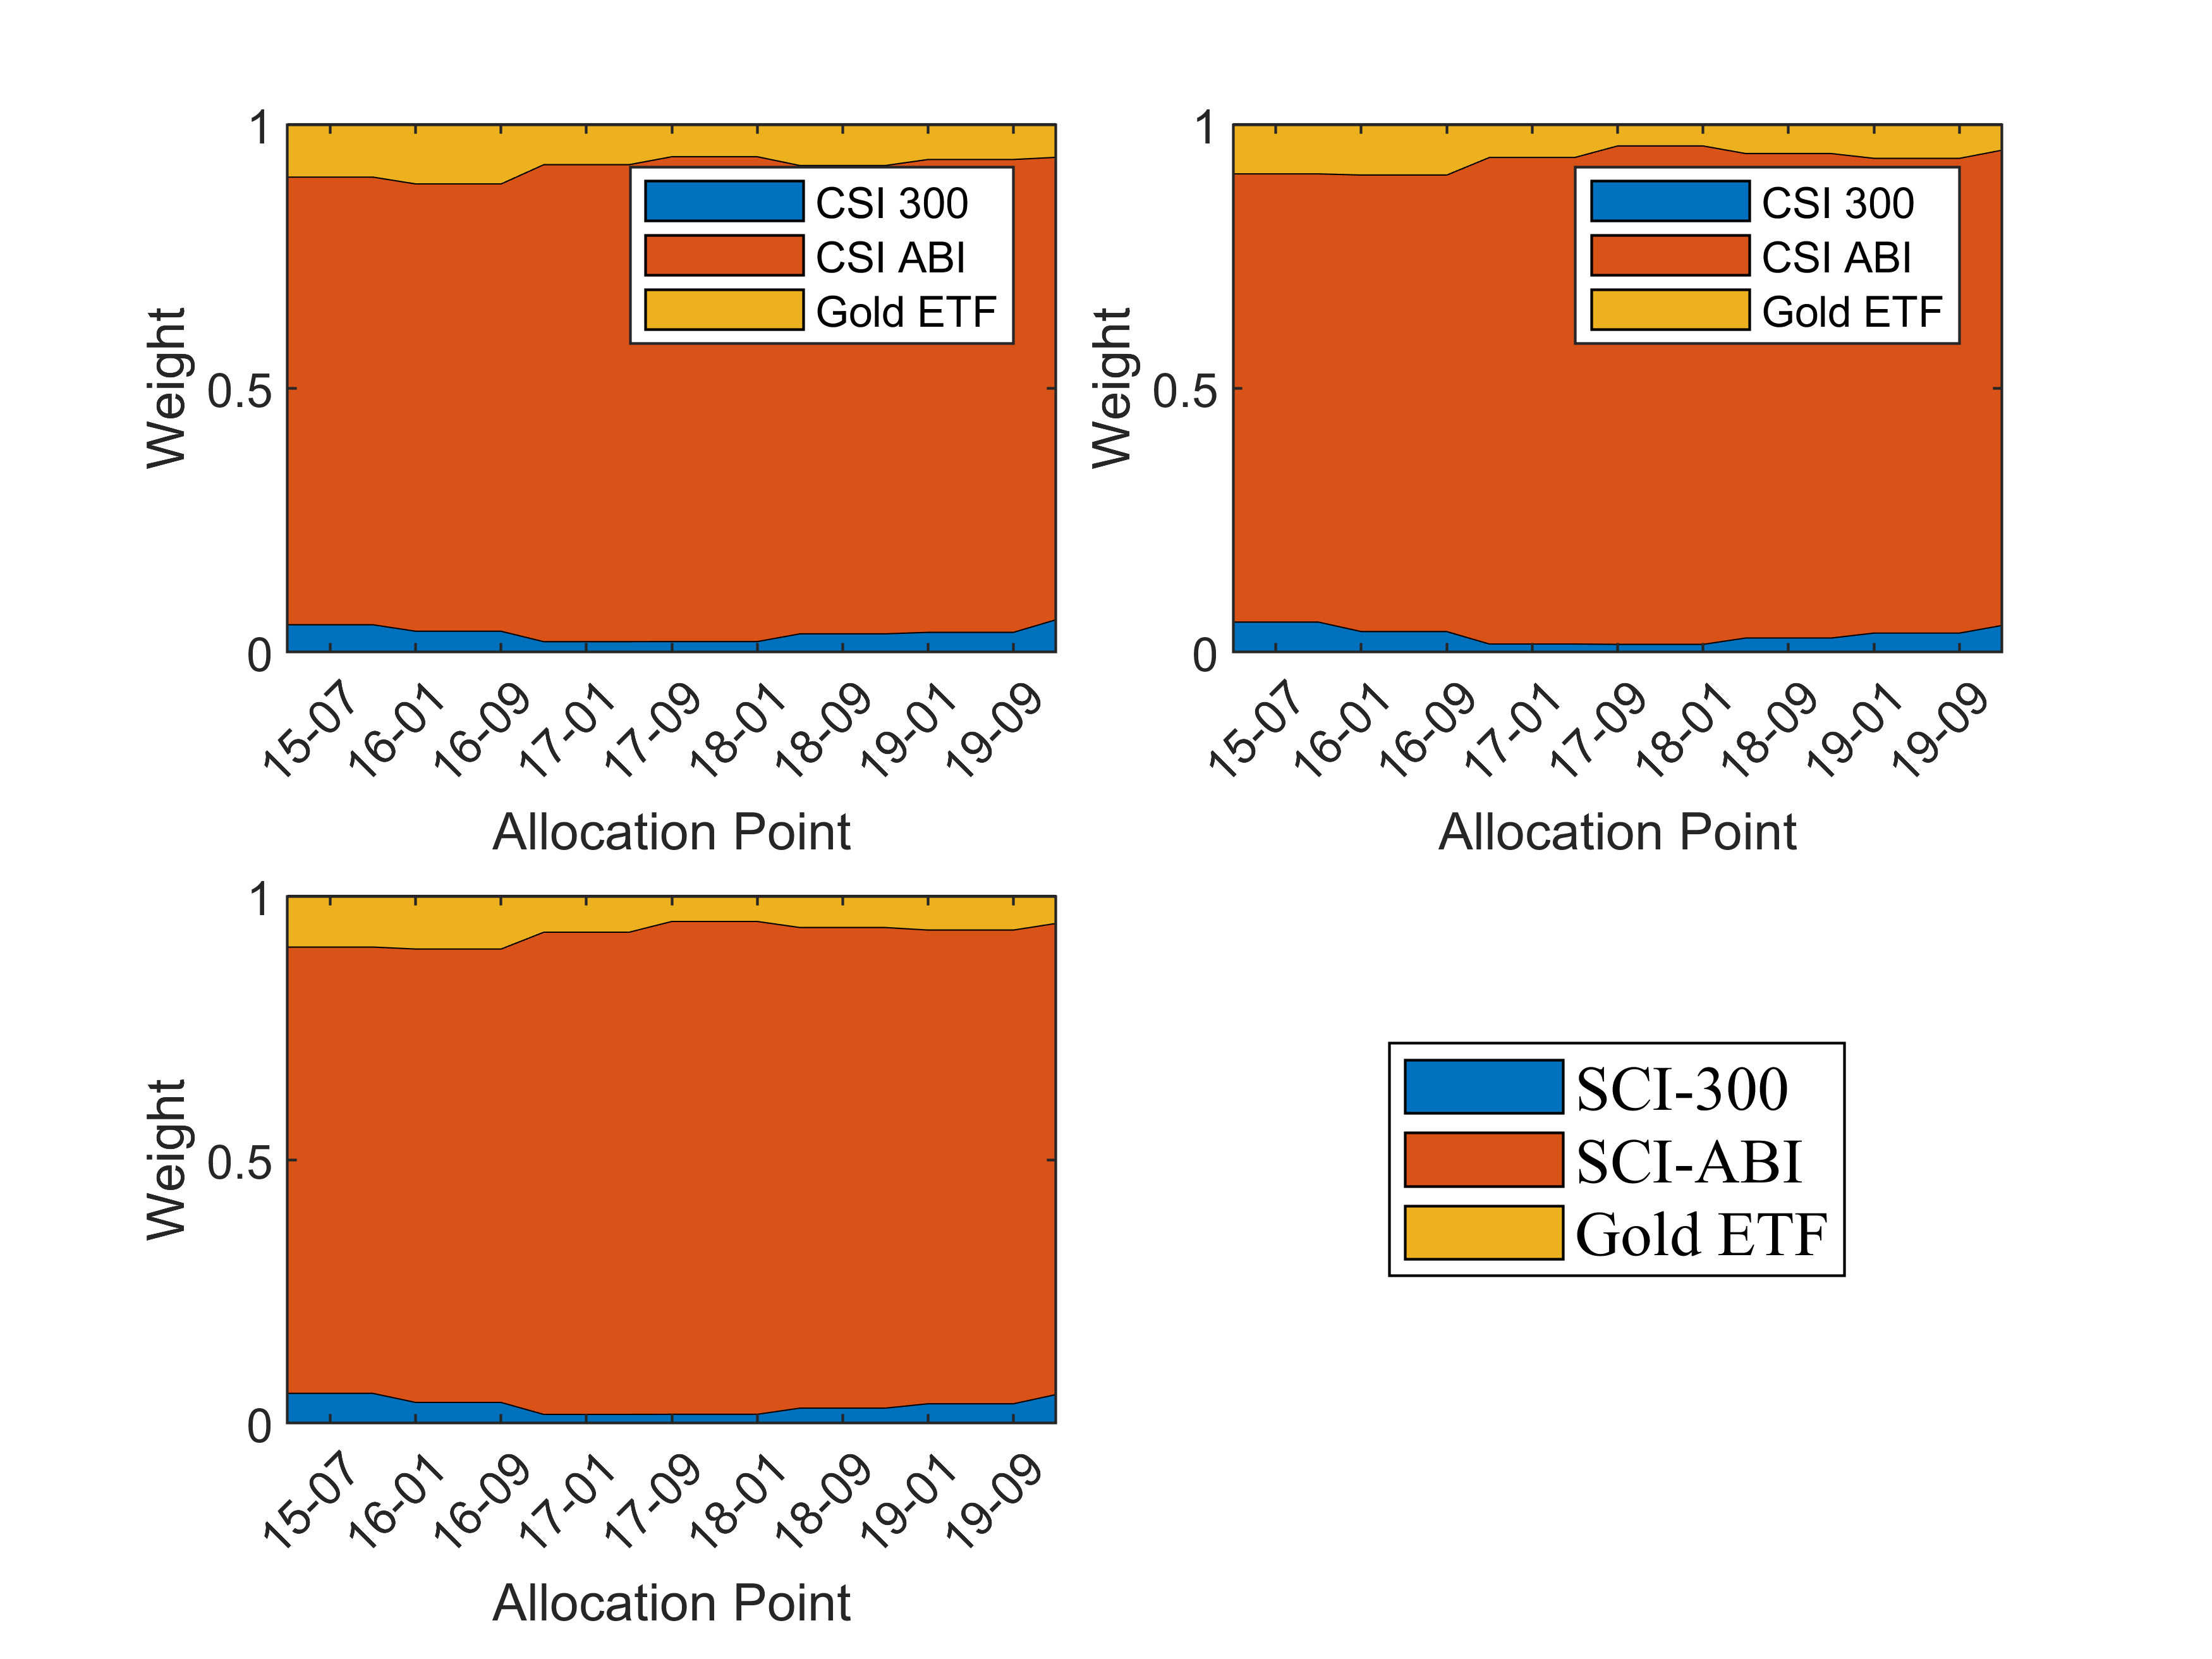
\includegraphics[scale=0.9]{Figure/FIG5-Allocation_Weight.png}
    \caption{The weight of assets based on Std Model(upper left), VaR Model (upper right), and ES Model (lower left)}
    \label{Fig5}
\end{figure}

\subsubsection{Analysis and Evaluation}
\paragraph{Allocation Models all outperform Individual Assets}\mbox{}\\
From the various evaluation indicators in \textbf{Table \ref{Tab3}}, we can find that the three allocation models have the following characteristics: (1) The annualized rate of return is higher than that of CSI 300 and CSI ABI, and lower than gold ETF; (2) The annualized volatility is much lower than that of CSI 300 and gold ETF, while it is slightly higher than that of CSI ABI. The maximum drawdown rate is lower than that of all individual assets; (3) Sharpe ratio is significant higher than that of a single asset.
This shows that through the asset allocation, financial risks have been dispersed adequately, and the overall performance of the asset portfolio is significantly better than that of a single asset.

\paragraph{Different models have their own characteristics}\mbox{}\\
Compared with the standard deviation models, the performance of the VaR model and the ES model is basically the same, both have higher annual returns, lower volatility and maximum drawdown than the standard deviation model. With respect to the Sharpe ratio, the standard deviation model is the lowest and the expected shortfall model is the highest. This is because the standard deviation indicator treats downside risk and upside risk equally. In other words, the standard deviation model overestimates the risk level of financial assets during the rising period, so that it could miss the investment opportunities when the "bull market" comes. 


\paragraph{Weight allocation with more debt and less shares}\mbox{}\\
According to the average weights of the three models allocated on various assets during the backtest period shown in \textbf{Table \ref{Tab4}}, it can be seen that the average allocation ratio of the VaR model is the lowest in the CSI 300 Index and the gold ETF, and the highest in the CSI ASI. The expected shortfall model is more sensitive to the changes of the upward and downward trend, so the allocation weight of stocks and gold ETF are slightly higher than VaR model. Finally, we also found that among three models, all of them have shown a significant feature of asset allocation ratio having more bonds than stocks, which is consistent with the fluctuation characteristics of assets.


\clearpage
\bibliographystyle{apalike}
\bibliography{ref}
\end{document}
